%%%% Establishing the collapse period -- does not belong in results? 
% As fraudulent practices at Enron had been going on for years if not decades, there is no specific ``deception moment''. We focus on the brief period that precedes the bankruptcy, as language might be likely to change around this time of reckoning, and deception of shareholders and the public was at its conscious peak. 
% The first signs of doubt appeared in the public space in the beginning of 2001 (cite WIKIPEDIA on ENRON scandal), leading up to the bankruptcy filing at the end of the same year (on December 2nd). We take October 2001 to be the beginning of the collapse, since it is at that time that the signs were apparent to the public (Enron's stock price started decreasing sharply, never to recover, and the company's credit rating was downgraded) and simultaneously, internal deception was provably practiced (Enron's legal council had requested auditors to destroy documents). %We therefore turn our attention to the beginning of October 2001. 

% The first signs of doubt appeared in the public space in the beginning of 2001, leading up to the bankruptcy filing on December 2nd of that year. We take October 2001 to be the beginning of the collapse since this was when it went public, and simultaneously, internal deception was provably practiced (Enron's legal council had requested auditors to destroy documents). 

Figures \ref{fig:politeness}, \ref{fig:discourse} and \ref{fig:sentiment} show the politeness, planning discourse, and sentiment levels respectively  in emails of the POIs, executives, and normal employees. 

The politeness of the execs and regular employees appeared to remain more or less constant throughout. However, in the POI emails, there was a distinct increase in politeness prior to the collapse, followed by a sharp drop thereafter, confirming the results in \cite{diplomacy}. 

\begin{figure}[b!]
    \centering
    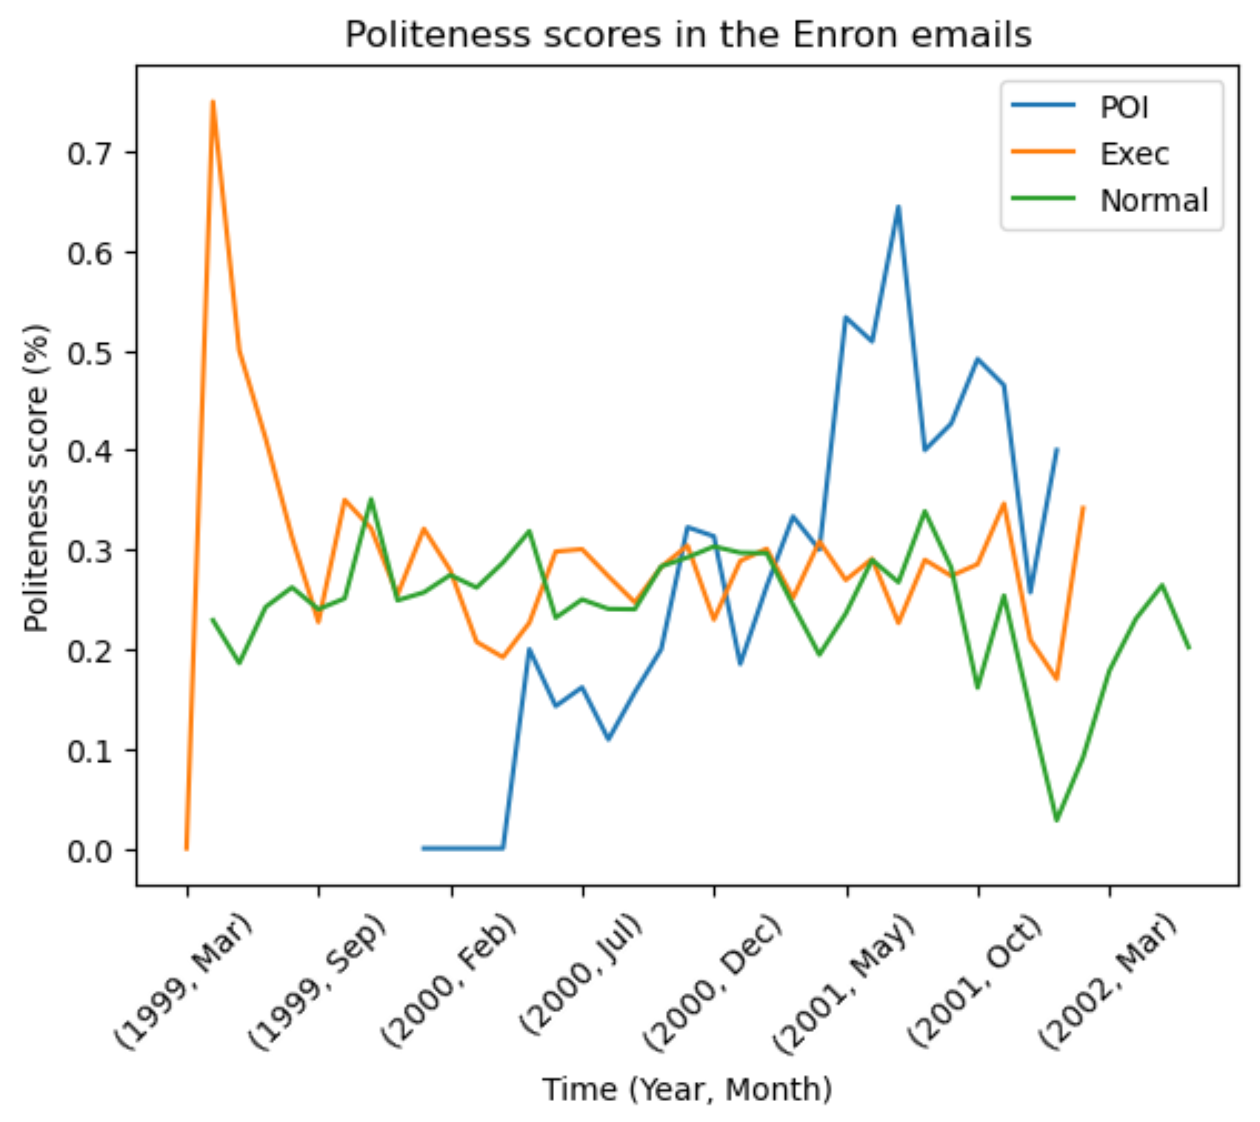
\includegraphics[width=8cm]{images/politeness_plot.png}
    \caption{Politeness scores produced by the Stanford politeness classifier}
    \label{fig:politeness}
\end{figure}

\begin{figure}[b!]
    \centering
    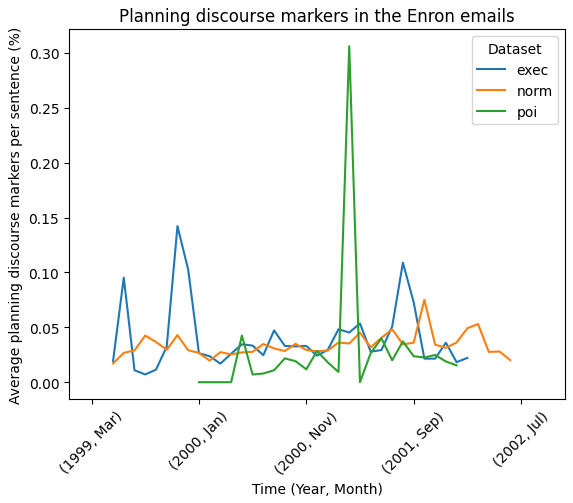
\includegraphics[width=8cm]{images/discourse_plot.png}
    \caption{Percentage of planning discourse markers per sentence in the Enron emails}
    \label{fig:discourse}
\end{figure}

The planning discourse frequencies in Figure \ref{fig:discourse} similarly showed a concordance with the features in \cite{diplomacy}. There is a clear spike in planning discourse which happens in March 2001 -- a time that coincides with the first public questioning of Enron's solvency in a \textit{Fortune} article \cite{fortune}. While it is impossible to assert a causal relationship, it should be noted that all data anomalies observed do line up with major events in the Enron collapse, and are isolated to only POI emails and not the general executive emails. %Similarly to Figure \ref{fig:politeness}, the trends for normal employees and executives appear to remain relativity stable compared to the POI results.

Figure \ref{fig:sentiment} did show a departure from the findings of \cite{diplomacy} where no clear increase in positive sentiment among the POI emails was seen. %In fact, the plot seemed to show a slight downward trend in sentiment for the POIs, a slight increase in sentiment for the normal employees, and a consistent sentiment for the other executives. 

Table \ref{tab:best_model_metrics} gives the model parameters and evaluation metrics for the best performing classifier trained. As seen, the model was competent at identifying POIs. This is promising given the presence of other executives in the data, and thus shows the models are able to identify features pertinent to POIs but not executives more broadly.

Figure \ref{fig:features} shows those features that were most useful for detecting fraudulent activity. %It is doubtful that a specific words (e.g., `ensure') would be indicators of a person's deceitful intentions, however 
Several features (`dont', `however', `doesnt') seemed to suggest a pattern of negative sentiment may be related to fraud, however it is interesting to note that this was not reflected in Figure~\ref{fig:sentiment}%, and therefore while these particular words may be related to detecting frauds, negative sentiment in general does not appear to be useful. However further work may be required to confirm this.

% \begin{figure}[t!]
%     \centering
%     \begin{subfigure}[b]{0.4\textwidth}
%         \centering
%         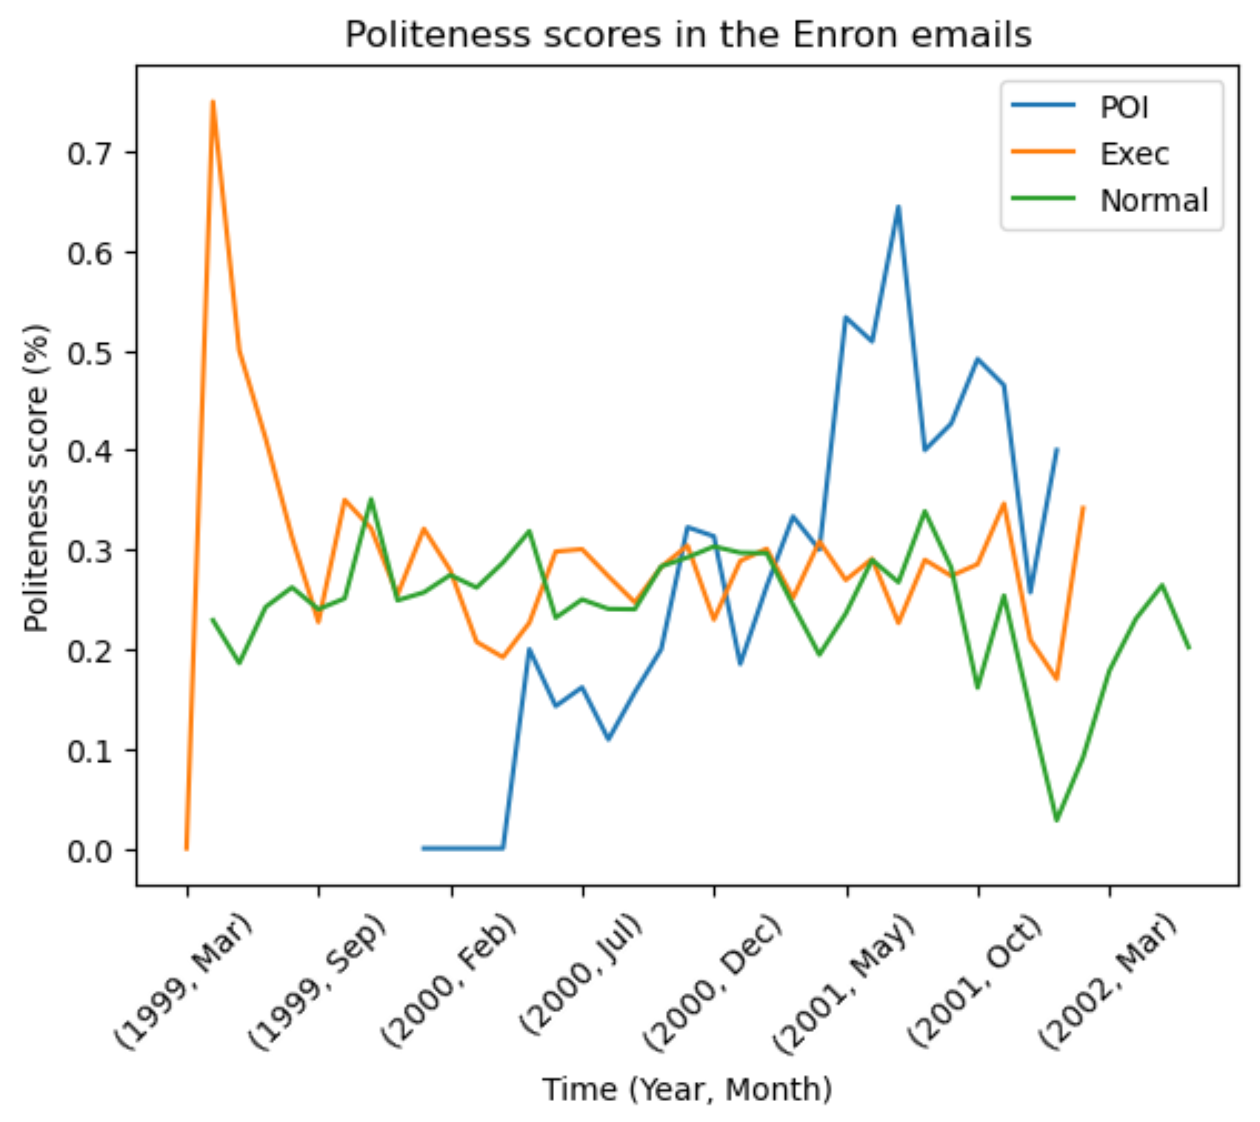
\includegraphics[width=8cm]{images/politeness_plot.png}
%         \caption{Politeness scores produced by the Stanford politeness classifier}
%         \label{fig:politeness}
%     \end{subfigure}
%     \begin{subfigure}[b]{0.4\textwidth}
%         \centering
%         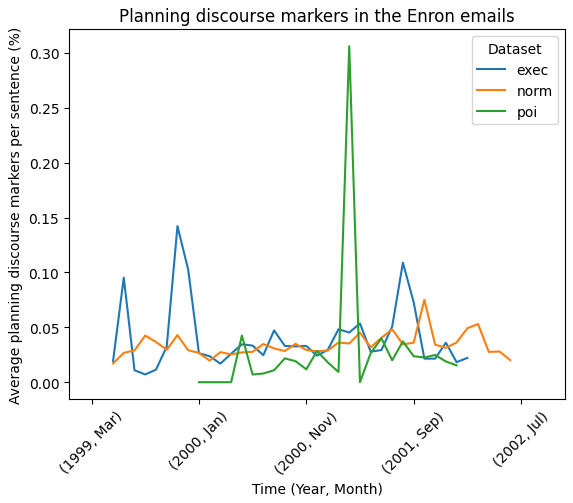
\includegraphics[width=8cm]{images/discourse_plot.png}
%         \caption{Need caption...}
%         \label{fig:discourse}
%     \end{subfigure}
%     \caption{Planning discourse markers in Enron emails}
%     \label{fig:politeness_discourse}
% \end{figure}


\begin{figure}[t]
    \centering
    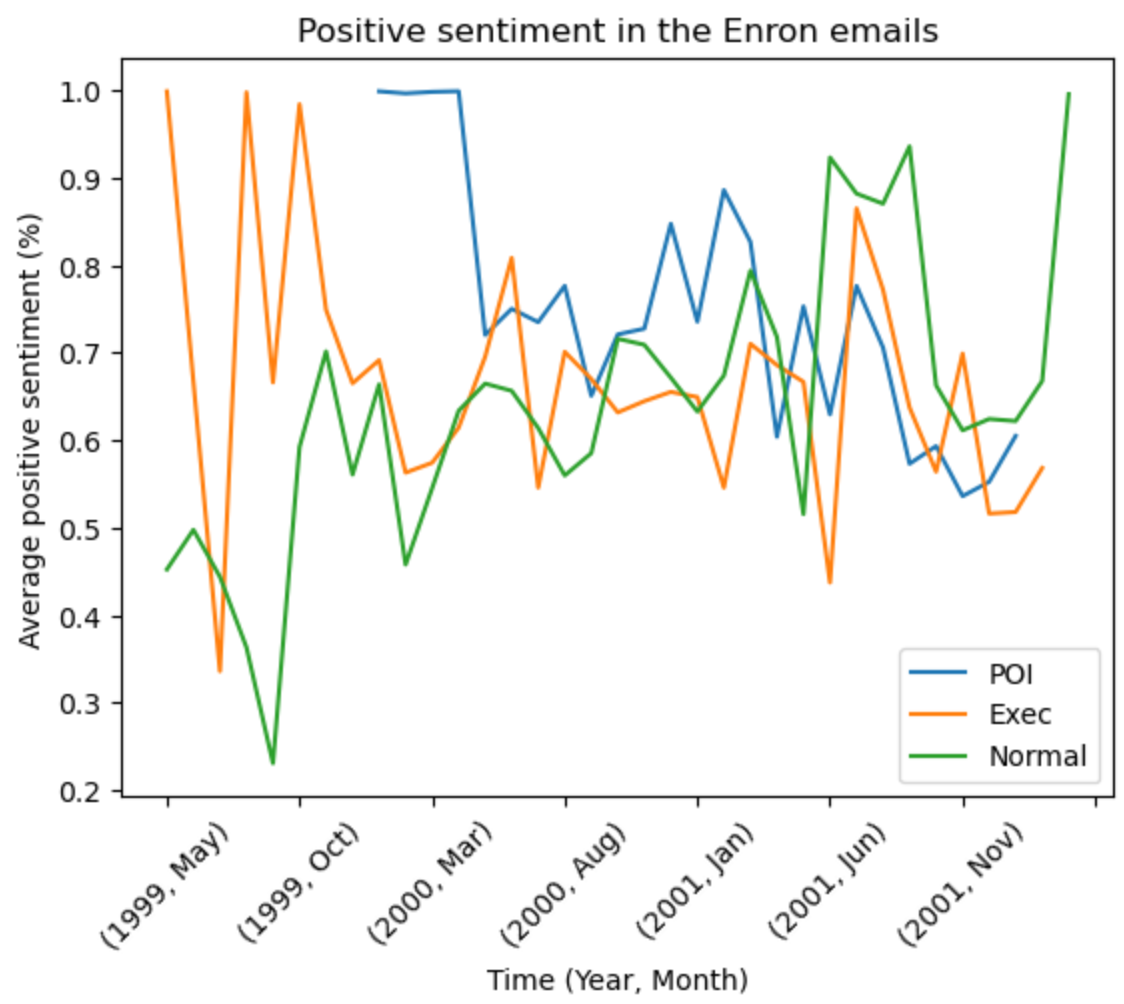
\includegraphics[width=8cm]{images/sentiment_plot.png}
    \caption{Sentiment fluctuation in Enron emails}
    \label{fig:sentiment}
\end{figure}

\begin{table}[b]
    \centering
    \begin{tabular}{|l|l|}
    \hline
    \textbf{Metric}            & \textbf{Value} \\ \hline
    Preprocessing               & Lemmatization + Unigram \\ \hline
    Model Class                & Logistic Regression (C=10) \\ \hline
    Precision         & 0.8204 \\ \hline
    Recall            & 0.8335 \\ \hline
    F1 Score          & 0.8170 \\ \hline
    Accuracy          & 0.8335 \\ \hline
    \end{tabular}
    \caption{Best Model Performance Metrics}
    \label{tab:best_model_metrics}
\end{table}

\begin{figure}[t!]
    \centering
    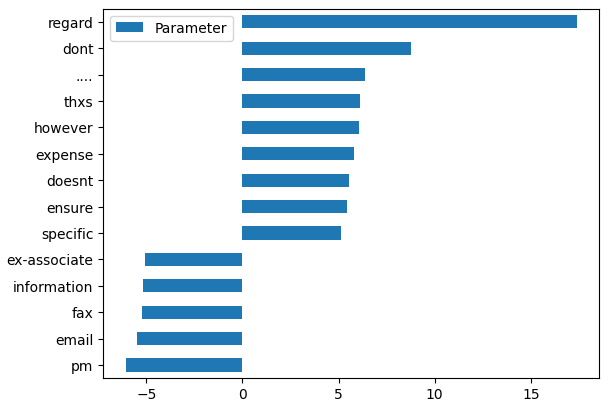
\includegraphics[width=8cm]{images/important_word_plot.png}
    \caption{Parameter weights for the top 14 features deemed most useful for detecting emails written by fraudulent/deceptive actors, as suggested by our best classifier}
    \label{fig:features}
\end{figure}

